\documentclass{sig-alt-release2}
\usepackage{graphics}

\begin{document}
% --- Author Metadata here ---
\conferenceinfo{SC'11 Companion,} {November 12--18, 2011, Seattle, Washington, USA.} 
\CopyrightYear{2011}
\crdata{978-1-4503-1030-7/11/11}
\clubpenalty=10000
\widowpenalty = 10000
% --- End of Author Metadata ---

\title{Poster: Automatic Parallelization of Numerical Python Applications Using the Global Arrays Toolkit}

\auwidth=1.12\textwidth
\numberofauthors{2}
\author{
% 1st. author
\alignauthor
Jeff Daily\\
\affaddr{Pacific Northwest National Laboratory}\\
\affaddr{P.O. Box 999}\\
\affaddr{MS K7-90}\\
\affaddr{Richland, WA}\\
\email{jeff.daily@pnnl.gov}
% 2nd. author
\alignauthor
Robert R. Lewis\\
\affaddr{School of Electrical Engineering and Computer Science}\\
\affaddr{Washington State University Tricities}\\
\affaddr{2710 Crimson Way}\\
\affaddr{Richland, WA 99354}\\
\email{bobl@tricity.wsu.edu}
%\and  % use '\and' if you need 'another row' of author names
}

\maketitle
% citations aren't typically found in an abstract, right?
\begin{abstract}
Global Arrays is a software system from Pacific Northwest National Laboratory
that enables an efficient, portable, and parallel shared-memory programming
interface to manipulate distributed dense arrays. The NumPy module is the de
facto standard for numerical calculation in the Python programming language, a
language whose use is growing rapidly in the scientific and engineering
communities. NumPy provides a powerful N-dimensional array class as well as
other scientific computing capabilities. However, like the majority of the core
Python modules, NumPy is inherently serial. Using a combination of Global
Arrays and NumPy, we have reimplemented NumPy as a distributed drop-in
replacement called Global Arrays in NumPy (GAiN). Serial NumPy applications can
become parallel, scalable GAiN applications with only minor source code
changes.  Scalability studies of several different GAiN applications will be
presented showing the utility of developing serial NumPy codes which can later
run on more capable clusters or supercomputers.
\end{abstract}

\category{D.1.3}{Programming Techniques}{Concurrent Programming}
\category{D.2.2}{Software Engineering}{Design Tools and Techniques}[software libraries, user interfaces]
%\category{D.2.8}{Software Engineering}{Metrics}
\category{E.1}{Data Structures}{arrays, distributed data structures}

\terms{Design, Performance}

\keywords{Global Arrays, PGAS, Python, NumPy, GAiN}

\section{Introduction}
Scientific computing with Python\cite{Ros90} typically involves using the
NumPy\cite{Oli06}  package.  NumPy provides an efficient multi-dimensional
array and array processing routines. Unfortunately, like many Python programs,
NumPy is serial in nature.  This limits both the size of the arrays as well as
the speed with which the arrays can be processed to the available resources on
a single compute node.

%For the most part, NumPy programs are written, debugged, and run in
%singly-threaded environments. This may be sufficient for certain problem
%domains. However, NumPy may also be used to develop prototype software. Such
%software is usually ported to a different, compiled language and/or explicitly
%parallelized to take advantage of additional hardware.

The Global Arrays (GA) toolkit \cite{Nie06,Pnl11} is a software system
from Pacific Northwest National Laboratory (PNNL) that enables an efficient,
portable, and parallel shared-memory programming interface to manipulate
physically distributed dense multidimensional arrays, without the need for
explicit cooperation by other processes. GA compliments the message-passing
programming model and is compatible with MPI\cite{Gro99a} so that the
programmer can use both in the same program. GA has supported Python bindings
since version 5.0. GA has been leveraged in several large computational
chemistry codes and has been shown to scale well \cite{Apr09}.

Global Arrays in NumPy (GAiN)\cite{Dai09,Dai11} is an extension to Python that
provides parallel, distributed processing of arrays. It implements a subset of
the NumPy API so that for some programs, by simply importing GAiN in place of
NumPy they may be able to take advantage of parallel processing transparently.
Other programs may require slight modification. This allows those programs to
take advantage of the additional cores available on single compute nodes and to
increase problem sizes by distributing across clustered environments.

\section{Approach}
The success of GAiN hinges on its ability to enable distributed array
processing in NumPy, to transparently enable this processing, and most
importantly to efficiently accomplish those goals. Performance Python
\cite{Ram08} ``perfpy'' was conceived to demonstrate the ways Python can be
used for high performance computing. It evaluates NumPy and the relative
performance of various Python extensions to NumPy. It represents an important
benchmark by which any additional high performance numerical Python module
should be measured. The original program \texttt{laplace.py} was modified by
importing \texttt{ga.gain} in place of \texttt{numpy} and then stripping the
additional test codes so that only the \texttt{gain} (\texttt{numpy}) test
remained.
%The latter modification makes no impact on the timing results since all tests
%are run independently but was necessary because \texttt{gain} is run on
%multiple processes while the original test suite is serial. 
The program was run on the chinook supercomputer at the Environmental
Molecular Sciences Laboratory (EMSL), part of Pacific Northwest National
Laboratory (PNNL). Chinook consists of 2310 HP DL185 nodes with dual socket,
64-bit, Quad-core AMD 2.2 GHz Opteron processors. Each node has 32 Gbytes of
memory for 4 Gbytes per core and a local scratch disk.
%Fast communication between the nodes is obtained using a single rail
%Infiniband interconnect from Voltaire (switches) and Melanox (NICs). The
%system runs a version of Linux based on Red Hat Linux Advanced Server.
GAiN utilized up to 512 nodes of the cluster, using 4 cores per node.

We noted during initial evaluations of \texttt{laplace.py} that the wall clock
time did not compare favorably with the timer for the solver. Figure
\ref{fig:laplace} quantifies this behavior using a strong scaling test of the
two timers. Although the solver is shown to scale up to 2K cores on a modest
problem size, the overall time to run the application exhibits inverse scaling.
Previous research \cite{Scu11,Man11} confirms our results and indicates the
problem is due to Python's excessive access of the file system during the
import of modules. In a serial environment, this is reasonable behavior. For a
shared filesystem on a cluster, all Python interpreters are thrashing the on
same module files.

\begin{figure}
\centering
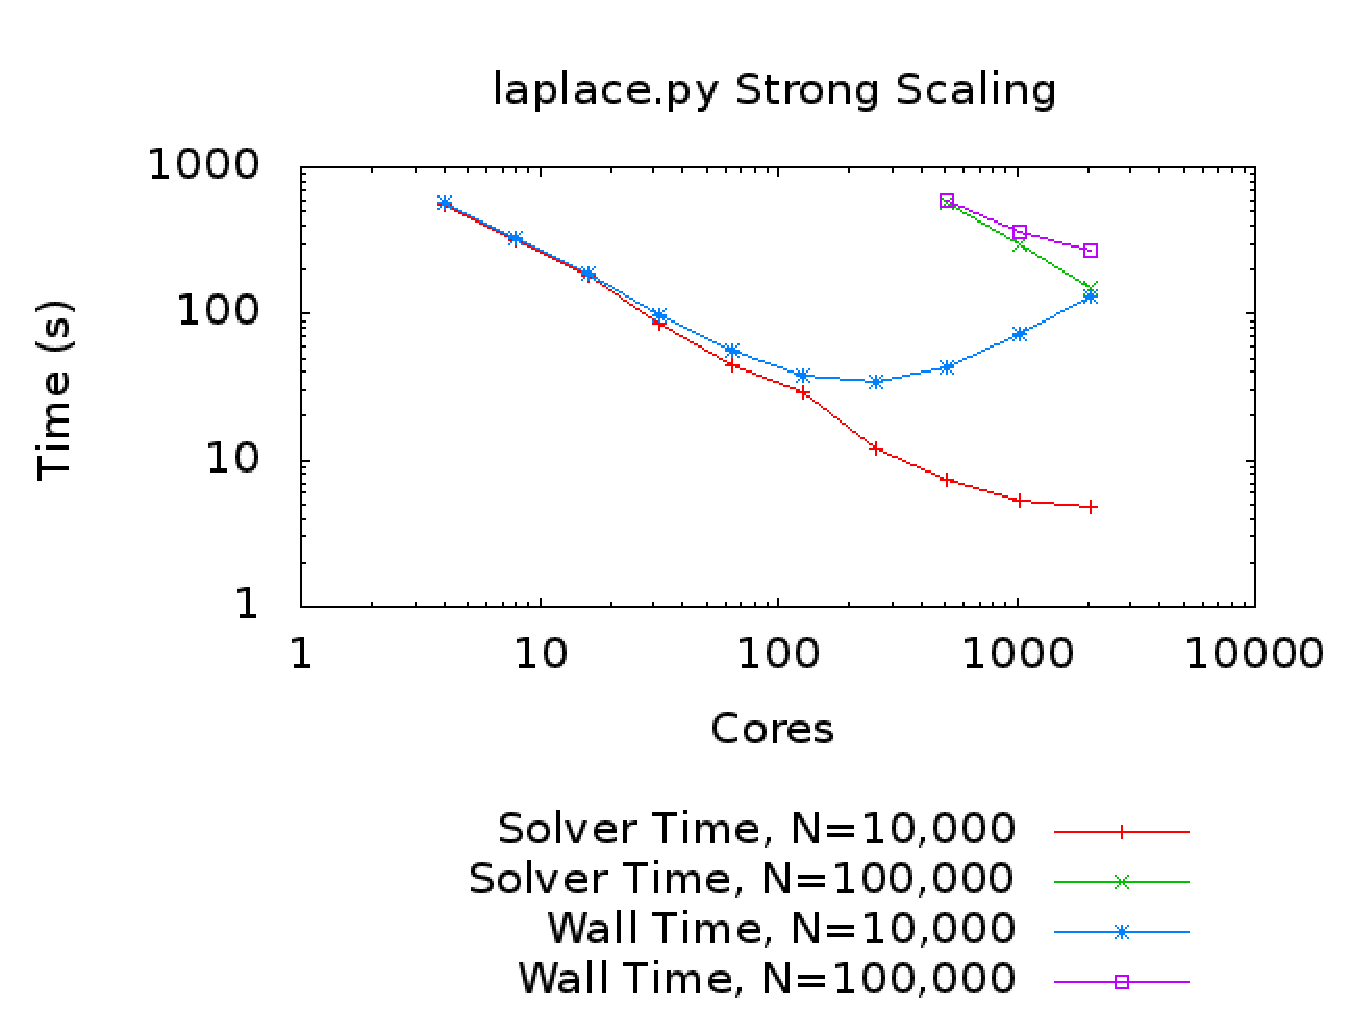
\includegraphics[width=0.48\textwidth]{laplace.eps}
%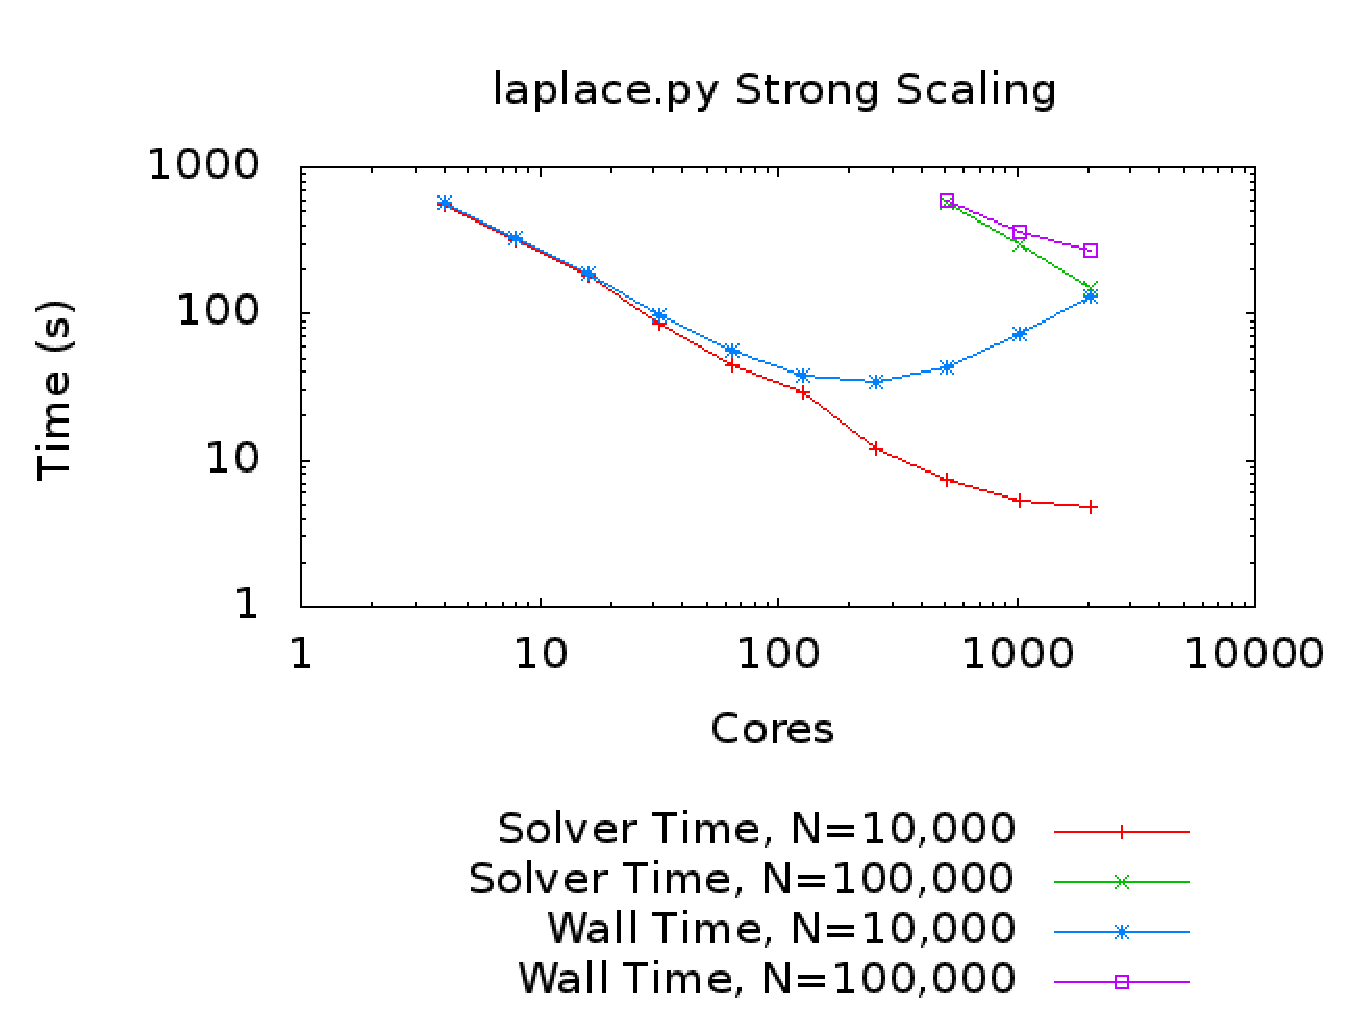
\epsfig{file=laplace,width=0.48\textwidth}
\caption{laplace.py Strong Scaling for 10K$^2$ Matrix}
\label{fig:laplace}
\end{figure}

Our solution to the problem is unique to clusters where the compute nodes have
local scratch disks such as EMSL's chinook system. The Python interpreter and
its associated modules and shared libraries are bundled and broadcast from node
zero to the remaining nodes, the master process on each node unbundles the
files, and the Python interpreter is run locally from each compute node. This
limits disk access to the local scratch disks where only eight processes
compete for the local filesystem. Our tests execute the simple Python program
``\texttt{import numpy}''. Figure \ref{fig:python} compares the cost of running
a global-filesystem shared Python interpreter, the individual cost of the
broadcast, the individual cost of running a node-local Python interpreter, as
well as the cumulative cost of the proposed solution. The proposed solution
performs better than the global filesystem case.

\begin{figure}
\centering
\includegraphics[width=0.48\textwidth]{python.eps}
%\epsfig{file=python,width=0.48\textwidth}
\caption{`import numpy' Strong Scaling}
\label{fig:python}
\end{figure}

\section{Conclusion}
GAiN succeeds in its ability to grow problem sizes beyond a single compute
node. The performance of the perfpy code and the ability to drop-in GAiN
without modification of the core implementation demonstrates its utility. However, the scalability of the Python interpreter on a cluster using a shared filesystem limits the utility of Python. Our proposed solution, as well as the related solutions\cite{Scu11,Man11}, alleviate the cost of using Python at scale until a more robust solution can be found.

\section{Acknowledgments}
A portion of the research was performed using the Molecular Science Computing
(MSC) capability at EMSL, a national scientific user facility sponsored by the
Department of Energy's Office of Biological and Environmental Research and
located at Pacific Northwest National Laboratory (PNNL). %PNNL is operated by
%Battelle for the U.S. Department of Energy under contract DE-AC05-76RL01830.

%
% The following two commands are all you need in the
% initial runs of your .tex file to
% produce the bibliography for the citations in your paper.
\bibliographystyle{abbrv}
\bibliography{post174-daily}
% You must have a proper ".bib" file
%  and remember to run:
% latex bibtex latex latex
% to resolve all references
%
% ACM needs 'a single self-contained file'!
%
% That's all folks!
\end{document}
